\subsection{Kết quả đo trên máy thực nghiệm}
Số tham số được tối ưu là 1,605,632, trên tổng 1,722,180,608 tham số. Checkpoint được chọn ở epoch 3. Loss validation của mô hình nền là 1.0810; giá trị tốt nhất sau tinh chỉnh là 0.0082. Thời gian ba epoch, gồm đánh giá validation và lưu checkpoint, là 1.97 phút. Bộ nhớ GPU cấp phát đỉnh do PyTorch ghi nhận là 3.93 GiB; số này không bao gồm toàn bộ bộ nhớ các ứng dụng khác.
\begin{figure}[htbp]\centering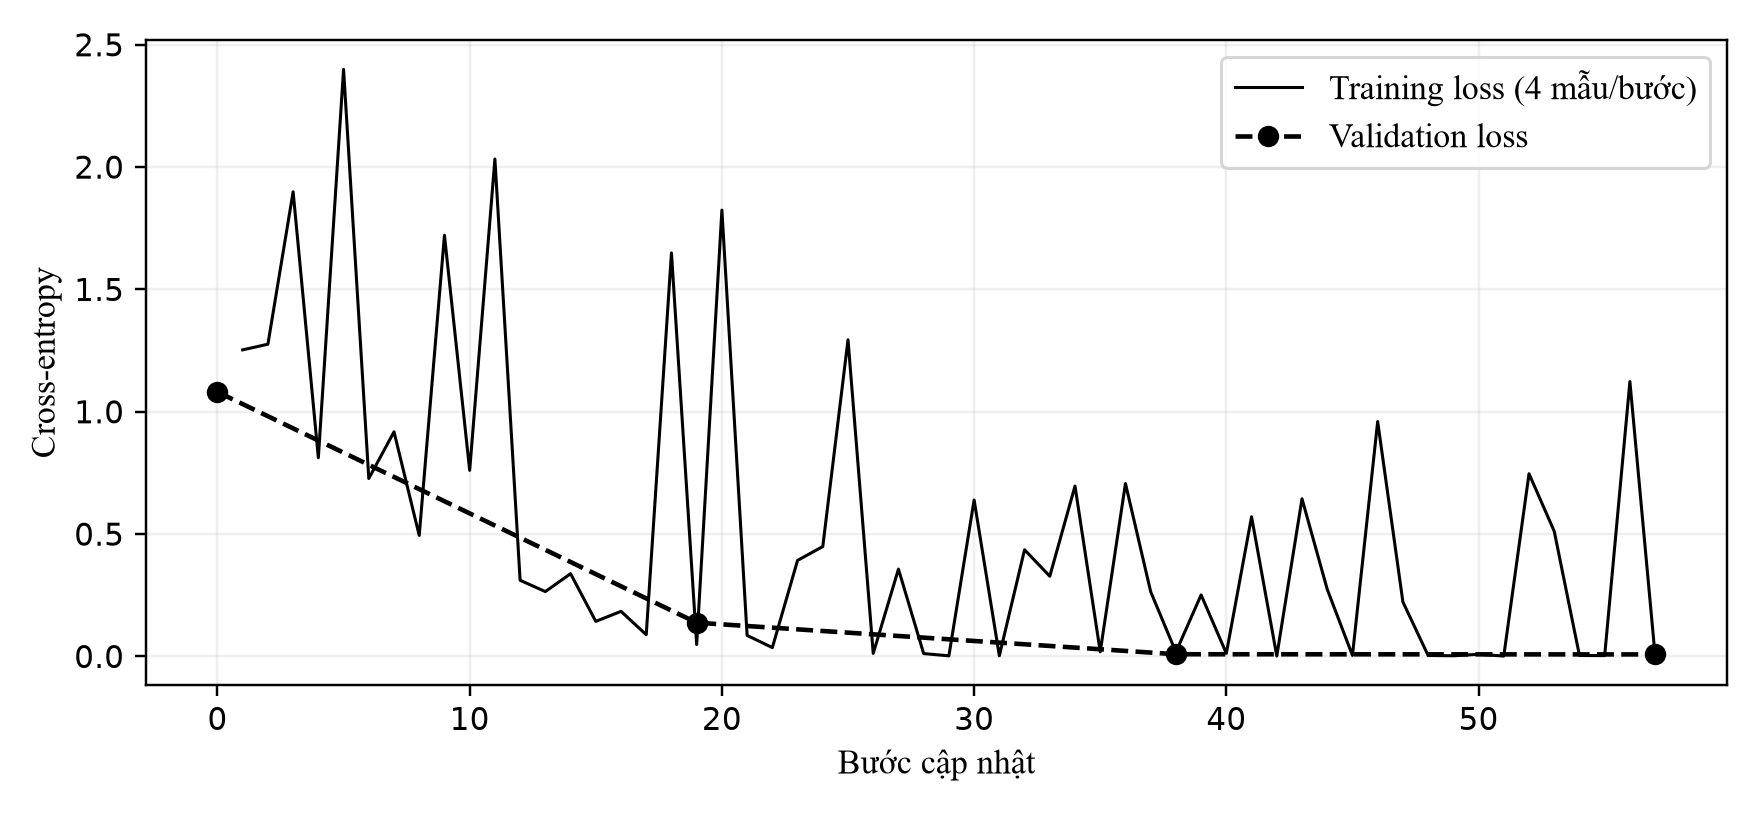
\includegraphics[width=\linewidth]{figures/qwen_learning.png}\caption{Loss huấn luyện theo bước và validation theo epoch. Điểm đầu validation thuộc mô hình nền.}\end{figure}
\begin{table}[H]\centering\small
\begin{tabular}{llrrrr}\toprule
Mô hình & Nhóm & Có dẫn mã & Mã lạ & Chạm giới hạn & Giây/câu\\\midrule
Qwen nền & Kiến thức & 0/8 & 0 & 0 & 8.07\\
Qwen nền & Hội thoại & 0/8 & 0 & 0 & 4.97\\
Qwen LoRA & Kiến thức & 8/8 & 0 & 0 & 7.57\\
Qwen LoRA & Hội thoại & 7/8 & 1 & 0 & 4.93\\
\bottomrule\end{tabular}
\caption{Kiểm tra hình thức đầu ra trên hai nhóm test, mỗi nhóm 8 câu.}\end{table}
Có dẫn mã chỉ kiểm tra sự xuất hiện của mã tài liệu, không chứng minh trích dẫn hỗ trợ đầy đủ câu trả lời. Mã lạ là mã không nằm trong ngữ cảnh đã cấp. Chạm giới hạn nghĩa là sinh đủ 320 token, có nguy cơ câu bị cắt. Độ trễ được đo sau khi mô hình đã nạp, không gồm thời gian khởi động hoặc truy xuất Neo4j. Hai mô hình dùng cùng ngữ cảnh được chỉ định trước để tách ảnh hưởng của bộ sinh; kết quả này chưa đo toàn bộ pipeline truy xuất.

Tệp \path{results/local_qwen/base_answers.json} và \path{results/local_qwen/lora_answers.json} lưu nguyên văn từng phản hồi. Tệp \path{results/local_qwen/training_summary.json} lưu cấu hình, mã băm dữ liệu và tài nguyên đo được. Các tệp này cho phép kiểm tra lại kết luận mà không cần dựa vào ảnh minh họa.
